\section{Experimental Results}
\label{sec:result}
We have implemented our approach within the \textsc{Singular} symbolic
algebra computation system [v. 3-1-6] \cite{DGPS}. Using our
implementation, we have performed experiments to verify two SMPO
architectures --- Agnew-SMPO \cite{agnew1991implementation} and the
RH-SMPO \cite{RHmulti} --- over $\Fkk$, for various datapath/field
sizes. Bugs are also introduced into the SMPO designs by modifying a
few gates in the combinational logic block. Experiments using SAT-,
BDD-, and AIG-based solvers are also conducted and results are
compared against our approach.  Our experiments run on a desktop with
3.5GHz Intel $\text{Core}^\text{TM}$ i7 Quad-core CPU, 16 GB RAM and
64-bit Linux.   

{\it Evaluation of SAT/ABC/BDD based methods:} To verify circuit $S$
against the polynomial $\F$, we unroll the SMPO over $k$ time-frames,
and construct a miter against a combinational implementation of $\F$.
A (pre-verified) $\Fkk$ Mastrovito multiplier \cite{mastro:1989} is
used as the {\it spec} model. This miter is checked for SAT using the
\emph{Lingeling} \cite{biere2013lingeling} solver. We also experiment
with the Combinational Equivalence Checking (CEC) engine of the ABC
tool \cite{abc}, which uses AIG-based reductions to identify internal
AIG equivalences within the miter to efficiently solve
verification. The BDD-based VIS tool \cite{brayton1996vis} is also used
for equivalence check. The run-times for verification of (unrolled)
RH-SMPO against Mastrovito {\it   spec} are given in Table
\ref{tbl:equiv} -- which shows that the techniques fail beyond 23 bit
fields.  

\vspace{-0.1in}
\begin{table}[htb]
\centering
\caption{\small Run-time for verification of bug-free RH-SMPO circuits
  for SAT, ABC and BDD based methods. \emph{TO} = timeout 14 hrs}
\label{tbl:equiv}
\begin{tabular}{|c||c|c|c|c|} 
\hline
& \multicolumn{4}{|c|}{Word size of the operands $k$-bits}  \\
\hline
Solver & 11 & 18 & 23 & 33 \\
\hline
\hline
Lingeling & 593  & \emph{TO}  & \emph{TO}  & \emph{TO}\\
\hline
\hline
ABC & 6.24 & \emph{TO} & \emph{TO} & \emph{TO}\\
\hline
\hline
BDD & 0.1 & 11.7 & 1002.4 & \emph{TO}  \\
\hline
\end{tabular}
\label{table:satbdd}  
\end{table} 

CEC between unrolled RH-SMPO and Agnew-SMPO also suffers the same fate
(results omitted). In fact, both SMPO designs are based on slightly
different mathematical concepts and their computations in all
clock-cycles, except for the $k^{th}$ one, are also different. These
designs have no internal logical/structural equivalencies, and
verification with SAT/BDDs/ABC is infeasible. Their dissimilarity is
depicted in Table \ref{tbl:fraig}, where  $N_1$ depicts the number of
AIG nodes in the miter prior to {\it fraig\_sweep}, and the nodes
after {\it fraiging} are recorded as $N_2$; so $\frac{N_1-N_2}{N_1}$
reflects the proportion of equivalent nodes in original miter, which
emphasizes the (lack of) \emph{similarity} between two designs.  

\begin{table}[htb]
\centering
\caption{\small Similarity between RH-SMPO and Agnew's SMPO}
\label{tbl:fraig}
\begin{tabular}{|c||c|c|c|c|} 
\hline
Size $k$ & 11 & 18 & 23 & 33 \\
\hline
$N_1$ & 734  & 2011  & 3285  & 6723\\
\hline
$N_2$ & 529 & 1450 & 2347 & 4852\\
\hline
Similarity & $27.9\%$ & $27.9\%$ & $28.6\%$ & $27.8\%$  \\
\hline
\end{tabular}\label{table:similarity}  
\end{table} 

{\it Evaluation of Our Approach:} Our algorithm inputs the circuit
given in BLIF format, derives RATO, and constructs the polynomial
ideal from the logic gates and the register/data-word description.  We
perform one $Spoly$ reduction, followed by the bit-level to word-level 
substitution, in each clock cycle. After $k$ iterations, the final
result polynomial $R$ is compared against the spec polynomial. The
run-times for verifying bug-free and buggy RH-SMPO and Agnew-SMPO are
shown in Table \ref{tbl:exp1} and Table \ref{tbl:exp2}, respectively. 
We can verify, as well as catch bugs in, up to 100-bit
multipliers. Beyond 100-bit fields, our approach is infeasible --
mostly due to the fact that the intermediate 
abstraction polynomial $R$ is very dense and contains high-degree
terms, which can be infeasible to compute. However, it should be noted
that if we do not use the proposed bit-level to word-level
substitution, and compute reduced \Grobner bases with RATO, then our
approach does not scale beyond 33-bit datapaths. 

\begin{table}[htb]
\centering
\caption{\small Run-time (seconds) for verification of bug-free and
  buggy RH-SMPO using our approach} 
\label{tbl:exp1}  
\begin{tabular}{|c||c|c|c|c|c|c|} 
\hline
Operand size $k$ & 33 & 51 & 65 & 81 & 89 & 99\\
\hline
\#variables & 4785 & 11424 & 18265 & 28512 & 34354 & 42372\\
\hline
\#polynomials & 3630 & 8721 & 13910 & 21789 & 26255 & 32373\\
\hline
\#terms & 13629 & 32793 & 52845 & 82539 & 99591 & 122958\\
\hline
\hline
Runtime(bug-free) & 112.6 & 1129 & 5243 & 20724 & 36096 & 67021\\
\hline
Runtime(buggy) & 112.7 & 1129 & 5256 & 20684 & 36120 & 66929\\
\hline
\end{tabular}
%\begin{minipage}{8cm}
%\def\arraystretch{1.5}\tabcolsep 2pt
%% \begin{tabular}{|c||c|c|c|c|c|} 
%% \hline
%% Operand size $k$ & 33 & 51 & 65 & 81 & 89 \\
%% \hline
%% \#variables & 4785 & 11424 & 18265 & 28512 & 34354\\
%% \hline
%% \#polynomials & 3630 & 8721 & 13910 & 21789 & 26255\\
%% \hline
%% \#terms & 13629 & 32793 & 52845 & 82539 & 99591 \\
%% \hline
%% %\hline
%% Runtime(bug-free) & 112.6 & 1129 & 5243 & 20724 & 36096 \\
%% \hline
%% Runtime(buggy) & 112.7 & 1129 & 5256 & 20684 & 36120\\
%% \hline
%% \hline
%% \end{tabular}
%% %\end{minipage}
\end{table}

\begin{table}[hbt]
\centering
\caption{\small Run-time (seconds) for verification of
  bug-free and buggy Agnew's SMPO our approach}
\label{tbl:exp2}
\begin{tabular}{|c||c|c|c|c|c|} 
\hline
Operand size $k$ & 36 & 66 & 82 & 89 & 100 \\
\hline
\#variables & 6588 & 21978 & 33866 & 39872 & 50300\\
\hline
\#polynomials & 2700 & 8910 & 13694 & 16109 & 20300\\
\hline
\#terms & 12996 & 43626 & 67322 & 79299 & 100100 \\
\hline
\hline
Runtime(bug-free) & 113 & 3673 & 15117 & 28986 & 50692 \\
\hline
Runtime(buggy) & 118 & 4320 & 15226 & 31571 & 58861\\
\hline
\end{tabular}
\end{table}


\section{Conclusions and Further Work}\label{sec:concl}
This proposal has described a method to verify sequential Galois field
multipliers over $\Fkk$ using computer algebra and algebraic geometry
based approach. As sequential Galois field circuits perform the
computations over $k$ clock-cycles, verification requires an efficient
approach to unroll the computation, and represent it as a canonical
word-level multi-variate polynomial. Using algebraic geometry, we show
that the unrolling of the computation at word-level can be performed by
\Grobner bases and elimination term orders. Subsequently, we show
that the complex \Grobner basis computation can be eliminated by means
of a bit-level to word-level substitution, which is implemented using
the binomial expansion over Galois fields and Gaussian
elimination. Our approach is able to verify up to 100-bit sequential
circuits, whereas contemporary techniques fail beyond 23-bit
datapaths.  

Our approach still has following limitations: first, it can only be applied
on XOR-rich circuits, while most industrial designs are AND-OR gates dominant;
second, it only uses naive bit-word abstraction based on functions of arithmetic
circuits, which will be inefficient when the function does not have a straightforward
expression (such as an implicit function); last but not least, Gr\"obner basis computation
in our improved approach still requires a very long time. To overcome these limitations,
further explorations are needed for my research. 

One way to further boost the efficiency is to adopt techniques from sparse linear algebra.
Analysis on experiment results shows major time consumption is on ``multi-division" part.
A matrix-based technique named as "F-4 style reduction" \cite{F4reduce} can speed up the procedure
dividing a low-degree polynomial with term-sparse polynomial ideal. 

We can also further expand our theory to sequential FSM implicit traversal. The sequential multiplier
verified in our experiment is actually a mealy FSM without primary inputs, i.e., we verify it through 
a single-chain implicit traversal. Our theory can also be applied when there are primary inputs -- a 
generic FSM.

Let us put following 2-bit FSM as an example. According to state transition graph (STG), we can get 
its gate-level implementation.
$\{s_0, s_1\}$ are state/pseudo inputs, $\{t_0,t_1\}$ are state/pseudo outputs, and we have a primary input (PI)  
$x$.
\begin{figure}[hbt]
\centering
\subfigure[State Transition Graph(STG)]{
\label{Fig.sub.1}
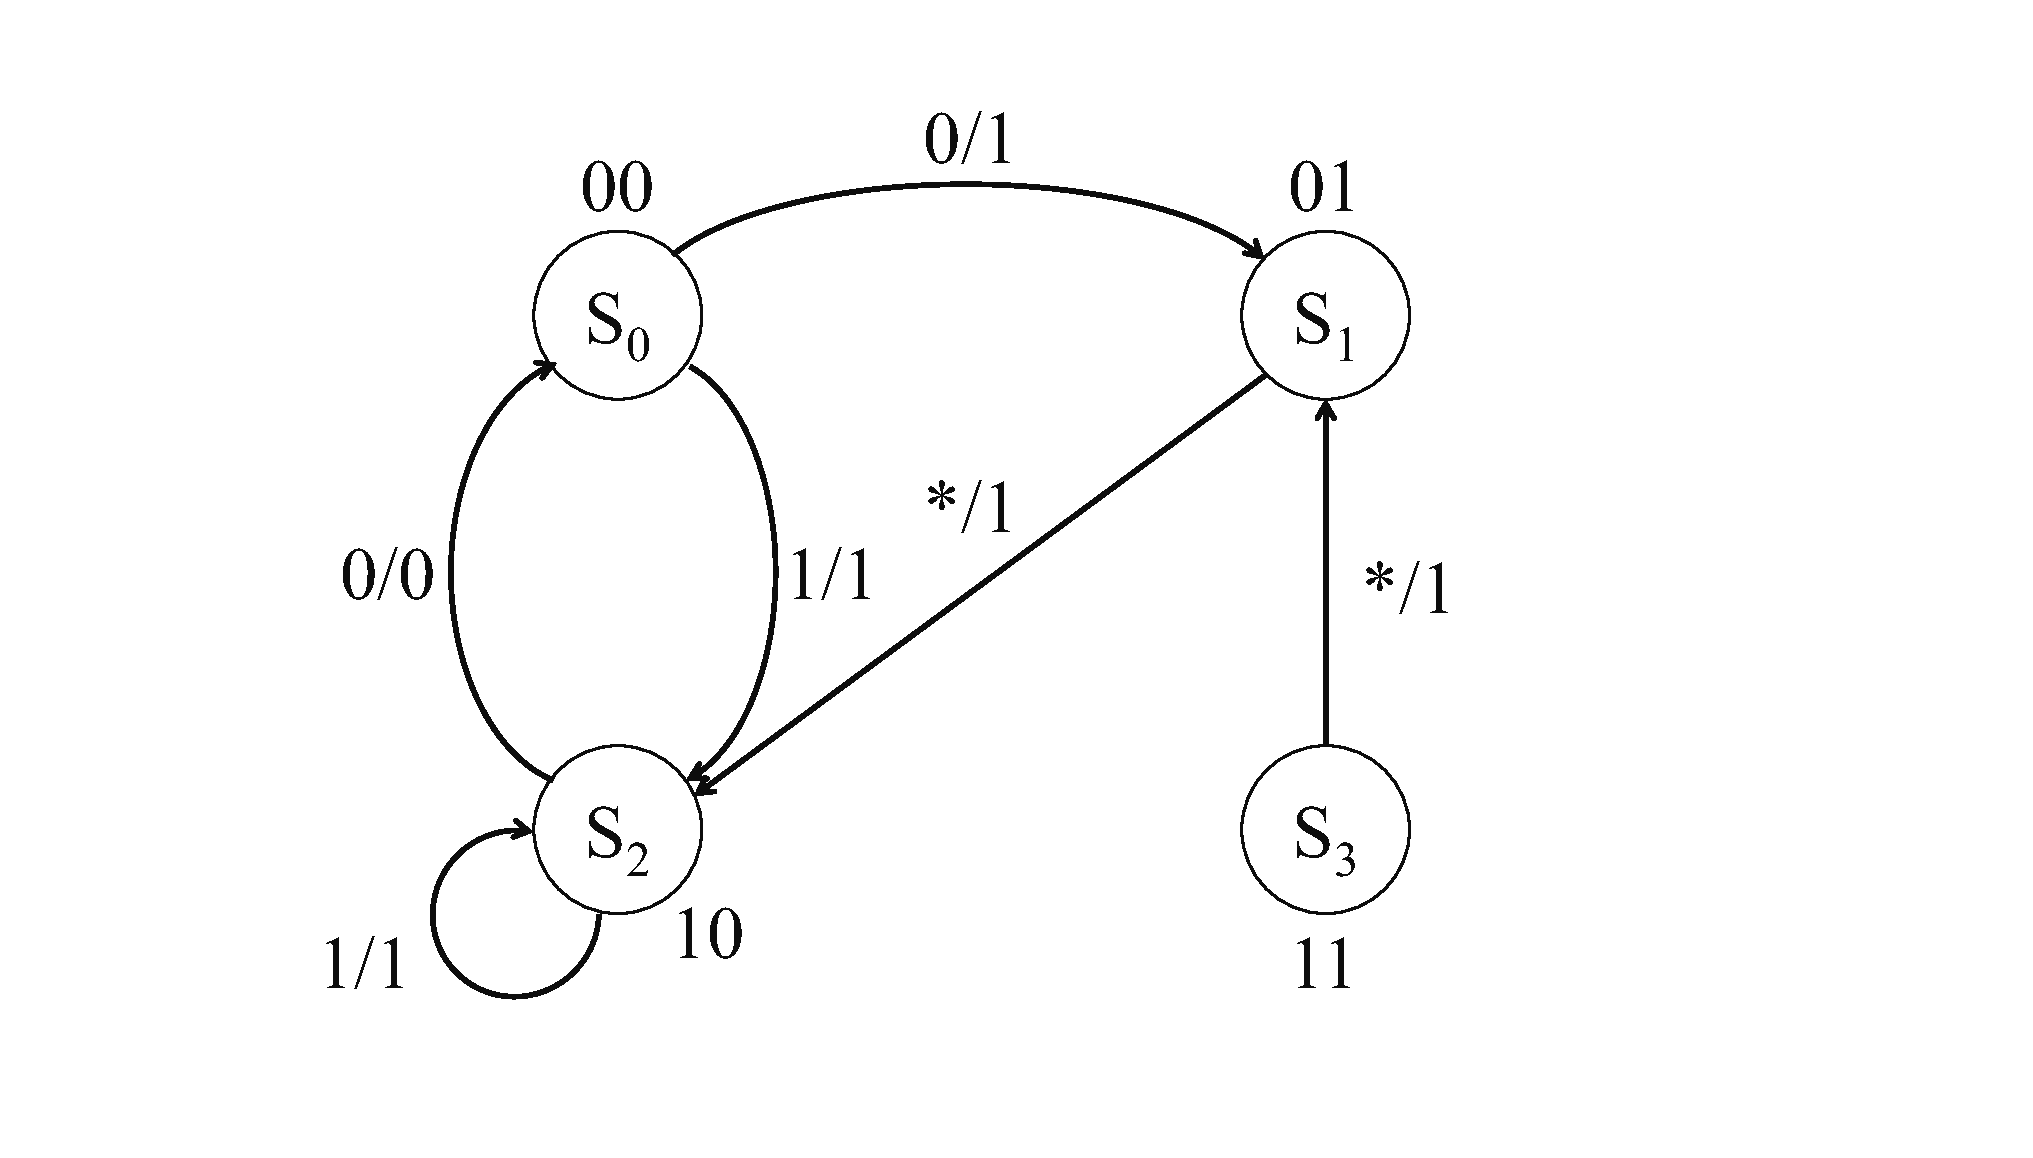
\includegraphics[width=0.35\textwidth]{stg_fig.eps}}
\subfigure[Gate-level implementation]{
\label{Fig.sub.2}
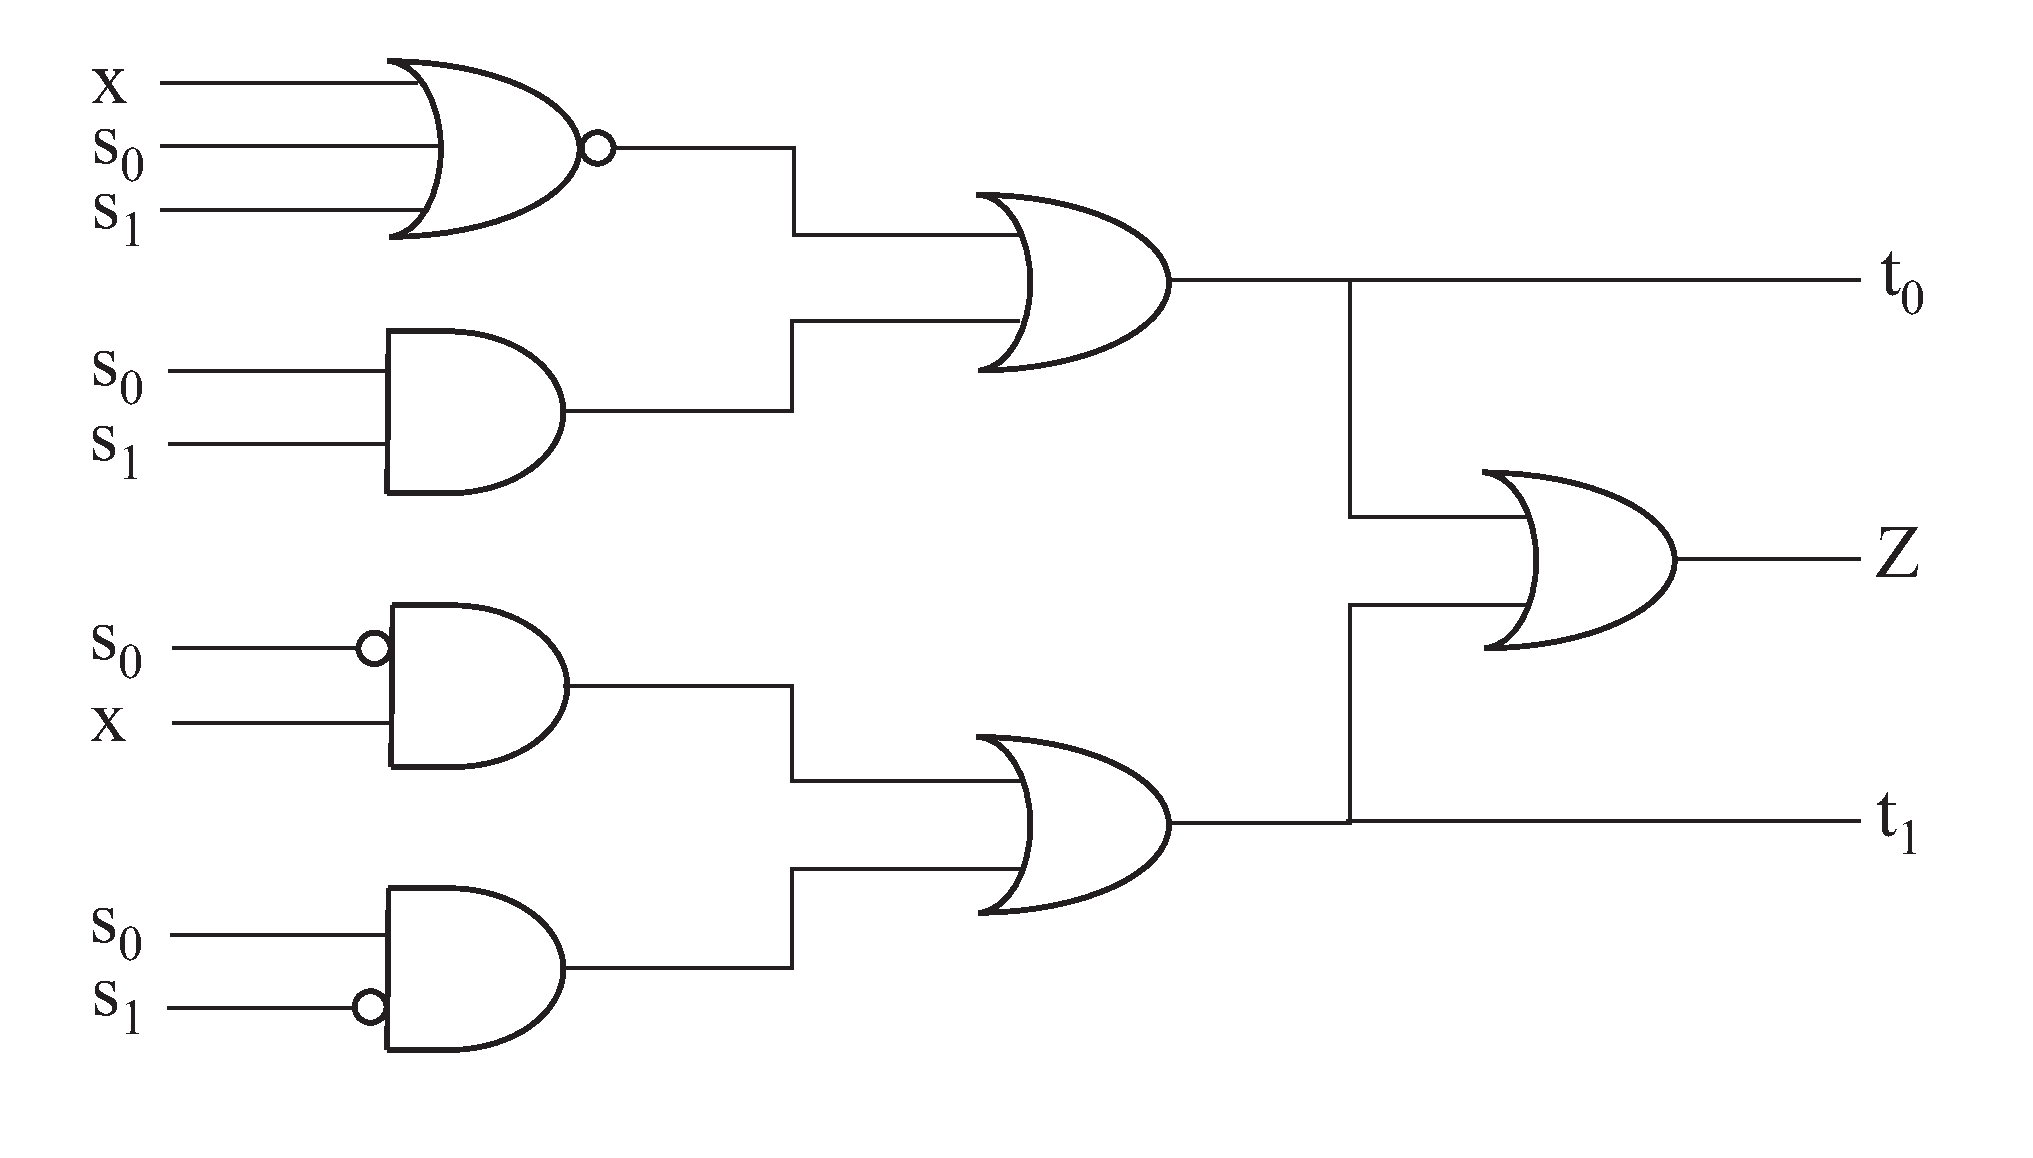
\includegraphics[width=0.55\textwidth]{fsm_fig.eps}}
\caption{Example Sequential Circuit}
\label{Fig.lable}
\end{figure}
Following algorithm is a modified breath-first search (BFS) traversal algorithm based on ideals with multivariate 
generators.
\begin{algorithm}[hbt]
\SetAlgoNoLine
 \KwIn{Transition polynomial $f_t = T + \mathcal F (S,x)$, 
	initial state ideal $from^0 = \langle S+\mathcal G(x), x^{q_1} - x\rangle$}

  $reached = from^0(T\setminus S)$\;
  \Repeat{$GB(new^i) == 1$}
  {
  	$i \gets i + 1$\;
	$to^i \gets$GB$(\langle f_t, from^{i-1}\rangle) \setminus \mathcal H(S)$\;
	$\overline{reached} = \langle T^{q_2}-T, x^{q_1} - x \rangle : reached$\;
	$new^i \gets $GB$(to^i + \overline{reached})$\;
  	$reached \gets $GB$( reached \cdot new^i)$\;
	$from^i \gets new^i(S\setminus T)$\;
  }
\Return{$reached$}
\caption {Algebraic Geometry based Traversal Algorithm (multivariate-generator ideals)}\label{alg:multi}
\end{algorithm}

Inputs of this algorithm are: a transition polynomial, which is the result of word-level abstraction; initial 
states description ideal, contains 2 generators defining PI could be any inputs and state inputs $S$ is a specific
value. (Ex: $\langle S+1+\alpha, x^2+x\rangle$ means initial state$=\{11\}$,
$\langle S+x\cdot\alpha, x^2+x\rangle$ means initial states$=\{00,10\}$).

Transition polynomial calculation exploits our improved RATO approach. After building
an elimination ideal, use RATO such that \emph{reverse\ topo\ order\ circuit\ variables }$> T > S > x$, the reduction
remainder has the form $T+\mathcal F(s_0,s_1,x)$. From word definition $S+s_0+s_1\alpha$ we get
$$s_0 = \alpha S^2+ (1+\alpha)S, s_1 = S^2+S$$
Do substitution, the transition polynomial of example circuit is 
$$f_T = T+S^3\cdot x+\alpha S^3+(1+\alpha)S^2\cdot x+S^2+S\cdot x+(1+\alpha)x+1$$

Assume we start from state $\{11\}$. First iteration, it will reach state $\{01\}$. Line 4 is to compose an
ideal with 2 generators from $from^0$ and transition polynomial $f_T$, compute its Gr\"obner basis. Note this ideal
has the form
\begin{equation}
I_{tran} = \left\{
             \begin{array}{c}
             T+\mathcal F(S,x) \\
             S + \mathcal G(x) \\
             v_x
             \end{array}  
        \right.
\end {equation}
$v_x$ is a polynomial containing only $x$, initially it should be vanishing polynomial $x^{q_1}-x$, with the program executing
it may be factorized.

Consider Buchberger's algorithm, all generators' leading terms are relatively prime, so it is a GB itself. 
Then we need to reduce this GB, we will find out $S + \mathcal G(x)$ could (possibly) be reduced by $v_x$,
and $T+\mathcal F(S,x)$ will definitely reduced by $S + \mathcal G(x)$. So, at last we will get a polynomial
$T + \mathcal F'(x)$ in reduce GB. We can include this polynomial and $v_x$, exclude the polynomial containing
$S$ (i.e. $\mathcal H(S)$ in algorithm), to compose an ideal representing \emph{next states} $to^i$. In iteration 1, result is $to^1 = \langle T+1, x^2+x\rangle$

Line 5 is the ideal quotient of universal set and reached states. In the first iteration, 
$reached$ is the initial state $\langle T+1+\alpha, x^2+x \rangle$. Result of ideal quotient
is $\langle T^3+(1+\alpha)T^2+\alpha T, x^2+x\rangle$ represents $\{00,01,10\}$.

Line 6 is ideals' sum (intersection of their varieties), it is done by combining all generators
from 2 ideals and compute GB. For first iteration result is $GB(\langle T+1,T^3+(1+\alpha)T^2+\alpha T, x^2+x\rangle) = \langle T+1, x^2+x\rangle$ representing $\{01\}$.

Line 7 is ideals' product (union of their varieties), it is done by multiplying all pairs of
generators from both ideal. For first iteration result is $GB(\langle (T+1)(T+1+\alpha),
(T+1)(x^2+x), (T+1+\alpha)(x^2+x), (x^4+x)\rangle) = \langle T^2+\alpha T+(1+\alpha), x^2+x\rangle$ representing $\{01,11\}$.

The traversal will run 3 iterations and terminate at 4th iteration. We list all intermediate 
results below:
\begin{itemize}
\item Iteration 1: $from^0 = \langle S+1+\alpha, x^2+x\rangle, to^1 = \langle T+1, x^2+x\rangle,
 reached = \langle T^2+\alpha T+(1+\alpha), x^2+x\rangle$
\item Iteration 2: $from^1 = \langle S+1, x^2+x\rangle, to^2= \langle T+\alpha, x^2+x\rangle,
reached = \langle T^3+1, x^2+x\rangle$
\item Iteration 3: $from^2 = \langle S+\alpha, x^2+x\rangle, to^3 = \langle T+\alpha x, x^2+x
\rangle, reached = \langle T^3\cdot x+x, T^4+T, x^2+x\rangle$
\item Iteration 4: $from^3 = \langle S, x\rangle, to^4 = \langle T+1, x\rangle, new = \langle1\rangle$
\end{itemize}
The final reachable states are represented by ideal $\langle T^3\cdot x+x, T^4+T, x^2+x\rangle$,
which means $\{00,01,10,11\}$.

This example shows a potential application of our proposed technique, which is promising if succeed on 
FSMs with larger word size and state numbers.